\documentclass{article}
\usepackage[utf8]{inputenc}
\usepackage{amsmath,amsfonts, amssymb, mathrsfs}
\usepackage[noabbrev, capitalise]{cleveref}
\usepackage[style=alphabetic, doi=false,isbn=false,url=false,  maxcitenames = 99, maxbibnames = 99]{biblatex}
\addbibresource{main.bib}
\usepackage{graphicx}
\usepackage{wrapfig}

\newcommand{\catname}[1]{{\normalfont\textbf{#1}}}
\newcommand{\Cat}{\catname{Cat}}
\newcommand{\LFP}{\catname{LFP}}
\newcommand{\SK}{\catname{Sk}}
\newcommand{\Rep}{\catname{Rep}}
\newcommand{\Surf}{\catname{Surf}}

\newcommand{\Sk}{\operatorname{Sk}}
\newcommand{\Free}{\operatorname{Free}}
\newcommand{\AW}{\operatorname{AW}}
\newcommand{\SL}{\operatorname{SL}}
\newcommand{\GL}{\operatorname{GL}}
\newcommand{\gl}{\mathfrak{gl}}
\newcommand{\slgroup}{\mathfrak{sl}}
\newcommand{\tr}{\operatorname{tr}_q}

\newtheorem{thm}{Theorem}
\newtheorem{prop}[thm]{Proposition}
\newtheorem{cor}[thm]{Corollary}
\newtheorem{conj}[thm]{Conjecture}
\newtheorem{qs}[thm]{Question}

\usepackage{fullpage}

% Uncomment to generate images from SVG
\usepackage[notransparent,inkscape=nolatex,inkscapearea=page,inkscapeformat=png]{svg}
\svgpath{{images/}{}}
\newcommand{\myincludesvg}[3]{\includesvg[#1,#2]{#3}}
\makeatletter
\newcommand{\myincludesvggroup}[4]{
\renewcommand\svg@ink@area{}%
\includesvg[#1,#2,inkscapename=#3-#4,inkscapeopt=-i #4 -j]{#3}%
\renewcommand\svg@ink@area{-C}%
}
\makeatother

% Uncomment to load statically generated images
%\newcommand{\myincludesvg}[3]{\includegraphics[#1]{svg-inkscape/#3_svg-raw.png}}
%\newcommand{\myincludesvggroup}[4]{\includegraphics[#1]{svg-inkscape/#3-#4_svg-raw.png}}

% skein pictures
\newcommand{\diagramhh}[4]{
\raisebox{-#3}{\myincludesvggroup{scale=0.25}{inkscape=nolatex,inkscapeformat=png,inkscapename=#1-#2,inkscapeopt=-i #2 -j}{#1}{#2}}\hspace{#4}%
}
\newcommand{\smalldiagram}[1]{\diagramhh{skeinrelations}{#1}{10pt}{1pt}}

\title{Research Statement}
\author{Juliet Cooke}
\date{December 2019}

\begin{document}

\maketitle

My research focuses on quantisation and categorification with applications in low dimensional topology, with a particular emphasis on bringing in contemporary tools from higher categories and homotopy theory to bear on the more classical theory of skein algebras.
First, I will survey my past research in this area, and then move to my current and future research directions.

\section{Past Research}
\subsection{Factorisation Homology and Skein Categories}

In my thesis I showed how skein algebras and skein categories can be computed by the mechanism of factorisation homology \cite{CookeThesis}. Firstly I recovered Kauffman bracket skein algebras of the four- punctured sphere and punctured torus from the locally finely presentable factorisation homology of the quantum group $\mathcal{U}_q(\slgroup_2)$ \cite{C1}. Generalising this result, I then showed that any skein category is a k-linear factorisation homology \cite{C2}.

\subsubsection{Factorisation Homology}

Factorisation homology is a recently developed method of constructing invariants of manifolds by associating to a disc an object $A$ in a monoidal $\infty$-category $\mathscr{C}^{\otimes}$ and ‘integrating’ the result over the manifold by taking the colimit over all the ways to embed discs into the manifold. It is a homology theory in the sense that it satisfies a generalisation of the Eilenberg–Steenrod axioms for singular homology \cite{AyalaFrancis2015}, and it can be used to construct (extended) topological quantum field theories (TQFTs) [Sch14]. 

Factorisation homology is a framework which encompasses many other homology theories and systems of constructing invariants of manifolds. A couple of simple examples are: if $\mathscr{C}^{\otimes}$ is the category of chain complexes and $A$ is an abelian group then the factorisation homology $\int^{\mathscr{C}}_M A$ simply recovers ordinary singular homology $H_{\bullet}(M)$; and if $A$ is an associative algebra then the factorisation homology of the circle $\int^{\mathscr{C}}_{S^1} A$ is the Hochschild homology $HH_{\bullet}(A)$. 

Building upon the works of \cite{david1}, I considered the factorisation homology where $A$ is a category of representations of a quantum group $\mathcal{U}_q(\mathfrak{g})$ and $\mathscr{C}^{\otimes}$ is either the $2$-category  $\Cat_k^{\times}$ of $k$-linear (enriched over $k$-vector spaces), small categories with the Cartesian product $\times$, or the $2$-category  $\LFP_k^{\boxtimes}$  of locally finitely presentable, $k$-linear categories with the Kelly-Deligne tensor product $\boxtimes$.

\subsubsection{Skein Algebras}

On the other hand, skein algebras are a generalisation of knot polynomials which were first developed in the 80s and give invariants of oriented surfaces. 
The typical example of a skein algebra is the Kauffman bracket skein algebra. The Kauffman bracket skein algebra of the oriented surface $\Sigma$ is the algebra of framed, oriented links in $\Sigma \times [0,1]$ modulo the local `skein relations'
\[
\smalldiagram{g4547} = q^{-1/2} \smalldiagram{g4563} + q^{1/2}\smalldiagram{g4571} \text{ and } \smalldiagram{g4617} = -q -q^{-1}.
\]
By introducing coupons and colouring, one may define a skein algebra $\Sk_G(\Sigma)$ for any reductive algebraic group G, or indeed any k-linear ribbon category $\mathscr{V}$. 

If one allows the tangles to have ends in $\Sigma \times \{0,1\}$ rather than always being closed one obtains the skein category $\SK_G(\Sigma)$ of Walker and Johnson-Freyd \cite{JohnsonFreyd19}: the objects are intervals in $\Sigma$ and the morphisms are the tangles. The skein algebra $\Sk_G(\Sigma)$ is then simply the endomorphism algebra of the empty set. 

\subsubsection{Main Result}
\begin{thm}\textup{\cite{C2}}  There is an equivalence of categories 
\[
\SK_G(\Sigma) \simeq \int_{\Sigma}^{\Cat_k^{\times}} \Rep^{fd}_q(G)
\]
between the $G$-skein category of the oriented surface $\Sigma$ and the factorisation homology of the surface with coefficients being $\Rep^{fd}_q(G)$ the category of finite dimensional representations of the quantum group $\mathcal{U}_q(\mathfrak{g})$.
\end{thm}

This makes precise a conjectured relation between skein algebras and the factorisation homology of quantum groups \cite{david1, JohnsonFreyd19}.

In order to prove this result I rely on the characterisation of factorisation homology in terms of its generalised Eilenberg–Steenrod axioms. In this case, this means that the factorisation homology $\int_{\_}^{\Cat_k^{\times}} \Rep^{fd}_q(G): \Surf^{or} \to \Cat_k^{\times}$ is the $2$-functor which assigns to a disc the category $\Rep^{fd}_q(G)$ and satisfies excision 
$$\int_{M \cup_{Z \times [0,1]} N}^{\Cat_k^{\times}} \Rep^{fd}_q(G) \simeq \int_{M}^{\Cat_k^{\times}} \Rep^{fd}_q(G) \times_{\int_{Z \times [0,1]}^{\Cat_k^{\times}} \Rep^{fd}_q(G) } \int_{N}^{\Cat_k^{\times}} \Rep^{fd}_q(G) $$
 such that the monodial structure of $\int_{Z \times [0,1]}^{\Cat_k^{\times}} \Rep^{fd}_q(G)$ is determined by the embedding of intervals. 

The proof then consists of two parts. The first part is understanding this relative tensor product. It is defined as the colimit in $\Cat_k^{\times}$ of the 2-sided bar construction, but I prove that this definition is equivalent to standard relative tensor of $k$-linear categories which has a straightforward categorical presentation \cite{Tambara01}. The second part is to use the categorical presentation of the relative tensor product to prove that skein category categories satisfy such an excision property and has a more topological flavour. 

\subsubsection{Corollaries}

If one takes the free-cocompletion of the skein category, this should be thought of as considering modules over the skein category, one recovers the $\LFP_k$ factorisation homology studied in \cite{david1}:

\begin{cor}\textup{\cite{C2}}
There is an equivalence of categories 
\[
\Free(\SK_G(\Sigma)) \simeq \int_{\Sigma}^{\LFP_k} \Rep_q(G) \simeq A_{\Sigma, G}-mod_{\Rep_q(G)}
\]
where $A_{\Sigma, G}$ is the Alekseev moduli algebra and has a combinatorial description in terms of the gluing pattern of $\Sigma$.
\end{cor}

The second equivalence is from \cite{david1}. Using this corollary we can return to skein algebras.

\begin{cor}\textup{\cite{C2}}
If $q$ is generic and $\Sigma$ is a punctured surface\footnote{There is a similar result possible for unpunctured surfaces.} then there is an isomorphism of algebras $\Sk_G(\Sigma) \cong A_{\Sigma}^{\mathcal{U}_q(\mathfrak{g})}$ between the skein algebra and the $\mathcal{U}_q(\mathfrak{g})$-invariant subgroup of $A_{\Sigma}$.  
\end{cor}

This gives a new way of approaching skein algebras which are easy to define but not easy to understand algebraically.
This also generalises an earlier result where this isomorphism was proven directly when $G=\SL_2$ and $\Sigma$ was the four-punctured sphere $\Sigma_{0,4}$ or once punctured torus $\Sigma_{1,1}$ \cite{C1}. 

\subsection{Spherical Double Affine Hecke Algebras \\ of Higher Genus}

This section outlines a joint work with Peter Samuelson which is currently being written up.
Double Affine Hecke Algebras (DAHAs) were introduced by Cherednik to prove Macdonald's constant term conjecture for Macdonald polynomials, and since then they have played an important role in representation theory and mathematical physics. 

\begin{wrapfigure}{r}{0.4\textwidth}
  \begin{center}
    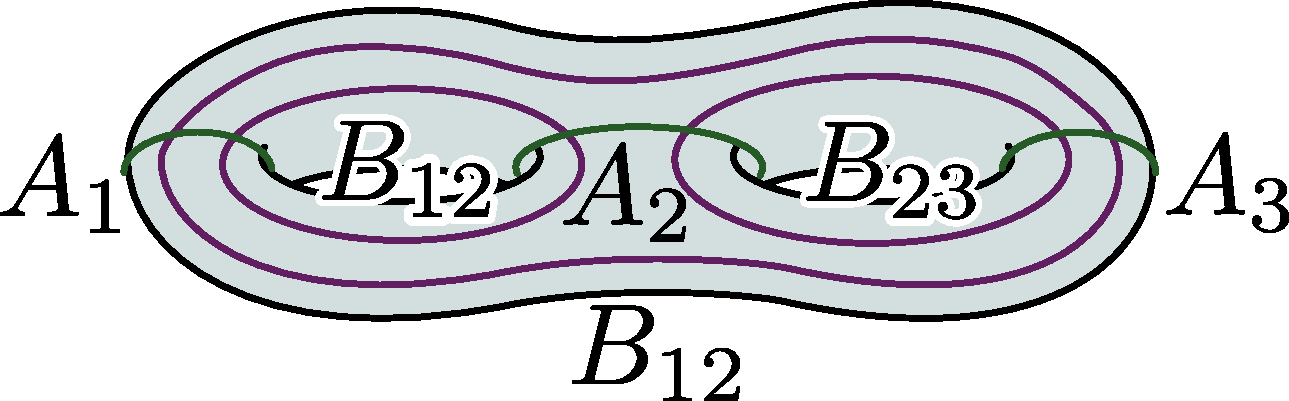
\includegraphics[width=0.38\textwidth]{2torus.pdf}
  \end{center}
  %\caption{The loops $A_1$, $A_2$, $A_3$, $B_{12}$, $B_{13}$ and $B_{23}$.}
\end{wrapfigure}
The spherical DAHA is a particular subalgebra which is know to be related to skein algebras: the spherical DAHA of type $C^{\vee}C_1$ is isomorphic to the Kauffman bracket skein algebra $\Sk_q(\Sigma_{0,4})$ of the four-punctured sphere, and the spherical DAHA of type $A_1$ quotient by a central element is isomorphic to the Kauffman bracket skein algebra $\Sk_q(\Sigma_{1,1})$ of the once puncture torus. Furthermore, the polynomial representation of the spherical DAHA of type $A_1$ is generated by two operators $\hat{\mathscr{O}}_A$ and $\hat{\mathscr{O}}_B$ which are associated to the $A$ and $B$ cycles of the torus. Arthamonov and Shakirov defined a generalisation $sH^{2}_q$ to a genus $2$ surface using six operators $\hat{\mathscr{O}}_{A_1}$, $\hat{\mathscr{O}}_{A_2}$, $\hat{\mathscr{O}}_{A_3}$, $\hat{\mathscr{O}}_{B_{12}}$, $\hat{\mathscr{O}}_{B_{13}}$ ,$\hat{\mathscr{O}}_{B_{23}}$ which act on $\mathscr{H}$, the space of Laurent polynomials in three variables which are symmetric under the $\mathbb{Z}^3_2$-group of Weyl inversions \cite{ArthamonovShakirov19}. 

We used the Masbaum--Vogel--Lickorish graphical calculus of $3$-valent graphs \cite{MasbaumVogel94, Lickorish93} to compute explicitly the actions of each loop on the skein module $\Sk(\mathcal{H}_2)$ of the solid $2$-handlebody $\mathcal{H}_2$ and concluded: 

\begin{thm}
The algebra of actions of the loops on $\Sk(\mathcal{H}_2)$ is isomorphic to the operator algebra $sH^2_q$ via an explicit change of basis map. 
\end{thm}

As well as giving a topological interpretation of the operator algebra $sH^2_q$, we can also conclude:

\begin{cor}
The operator algebra $sH^2_q$ contains two copies of the standard $A^1$ spherical DAHA and a copy of the $C^{\vee}C_1$ spherical DAHA given by the inclusions of surfaces. 
\end{cor}

\section{Current and Future Research}

\subsection{Dimensions of Skein Algebras}

The Alekseev moduli algebra $A_{\Sigma, G}$ has a natural grading by degree. As part of the direct proof that $\Sk_{\SL_2}(\Sigma) \cong A_{\Sigma}^{\mathcal{U}_q(\slgroup_2)}$ for $\Sigma = \Sigma_{0,4}$ or $\Sigma_{1,1}$, I computed the Hilbert series of  $A_{\Sigma}^{\mathcal{U}_q(\slgroup_2)}$ for these surfaces \cite{C1}. A Hilbert series encodes the dimensions of each graded part of an algebra $A = \bigoplus_{k \in \mathbb{Z}} A[k]$ as a series $h_A(t) = \sum_{k \in \mathbb{Z}} \dim(A[k]) t^k$.
I have recently found that this Hilbert series computation can be generalised as follows:
\begin{thm}
Let $\Sigma_{g,r}$ be the oriented surface of genus $g$ with $r>0$ punctures. The Hilbert series of the algebra of $\mathcal{U}_q(\slgroup_2)$-invariants $A_{\Sigma}^{\mathcal{U}_q(\slgroup_2)}$ graded by degree is 
\[
h(t) = \left(\frac{1+t}{1-t}\right)^n \left(\sum_{m=0}^{\infty} \left(\stackrel{n+m-1}{m} \right)^2 t^{2m} - \left(\stackrel{n+m-1}{m}\right) \left(\stackrel{n+m}{m+1}\right) t^{2m+1}\right)
\]
where $n = 2g+r-1$ is the number of handles in the handle decomposition of $\Sigma_{g,r}$. 
\end{thm}
\begin{conj}
The isomorphism $A_{\Sigma_{g,r}}^{\mathcal{U}_q(\slgroup_2)} \to \Sk_q(\Sigma_{g,r})$ is graded when $A_{\Sigma_{g,r}}^{\mathcal{U}_q(\slgroup_2)}$ is graded by degree and $\Sk_{\SL_2}(\Sigma_{g,r})$ is graded by the number of handles a loop goes around. 
\end{conj}
By grading the isomorphism between $A_{\Sigma_{g,r}}^{\mathcal{U}_q(\slgroup_2)}$ and the Kauffman bracket skein algebra $\Sk_{\SL_2}(\Sigma_{g,r})$, we could conclude that this is also the Hilbert series of $\Sk_{\SL_2}(\Sigma_{g,r})$. 

\begin{qs}
What is the Hilbert series for other Lie groups $G$?
\end{qs}

Of particular interest would be $G = \SL_n$ for higher $n$, as this case gives the Hompfy-pt skein algebras. Also as $\slgroup_n$ is still semisimple we still get a version of the Weyl character formula, so it is tractable to generalise the argument used for $\slgroup_2$. In order to treat this case as a straightforward generalisation, the first step would be to find the graded character of quantum loop algebra $\mathscr{O}_q(\SL_n)$, as the graded character of $A_{\Sigma_{g,r}, \SL_n}$ is simply this to the power of $n$. A vector space basis for $\mathscr{O}_q(M_n)$ is already known \cite{DomokosLenagan05}, and this should be useful in finding the graded character of $\mathscr{O}_q(\SL_n)$.
Another interesting case is $G = \GL_2$ which gives the $\gl_2$ web skein algebras \cite{QueffelecWedrich18}.

\subsection{Presentations of Skein Algebras}

The previous questions about the dimensions of skein algebras are motivative by a wider question; namely

\begin{qs}
What is a presentation of the Kauffman bracket skein algebra $\Sk_q(\Sigma_{g,r})?$
\end{qs} 

Despite skein algebras dating back to the 80s, presentations of Kauffman bracket skein algebras are only known for a handful of punctured surfaces: spheres with up to four punctures and tori with up to two punctures \cite{BullockPrzytycki00}. While it is not difficult to find relations between elements of a skein algebra it is difficult to conclude you have enough relations. The aim is to use the Hilbert series of $\Sk_q(\Sigma_{g,r})$ to prove I have enough relations.

Initially the aim is to answer this question for a few more examples such as the five punctured sphere $\Sigma_{0,5}$, the six punctured sphere $\Sigma_{0,6}$, or the punctured genus two surface $\Sigma_{2,1}$. The longer term goal is to use these new examples find a presentation for the general punctured case.

Bullock showed that $\Sk_q(\Sigma_{g,r})$ is generated by $2^n-1$ simple curves $ \{C\}$ with each generator uniquely determined by the handles of $\Sigma_{g,r}$ which it meets \cite{Bullock1999}. These simple curves should correspond to the quantum traces in $A_{\Sigma_{g,r}}^{\mathcal{U}_q(\slgroup_2)}$. 

\begin{conj}
\label{conj:IsomorphismMapsTrace}
The Algebra of $\mathcal{U}_q(\slgroup_2)$-invariants $A_{\Sigma_{g,r}}^{\mathcal{U}_q(\slgroup_2)}$ is generated by the quantum traces $\tr(X_{i_1} \dots X_{i_k})$ with $i_{j} < i_{j+1}$ and $i_k \leq n$, and  the isomorphism $A_{\Sigma_{g,r}}^{\mathcal{U}_q(\slgroup_2)} \to \Sk_q(\Sigma_{g,r})$ maps $\tr(X_{i_1} \dots X_{i_k})$ to the generator $s_{i_1 \dots i_k}$ of $\Sk_q(\Sigma_{g,r})$ which intersects the handles $i_1, \dots, i_k$. 
\end{conj}

If I find a set of generators $\{R\}$ such that the algebra $< C | R>$ has the same Hilbert series as  $\Sk_q(\Sigma_{g,r})$ then this algebra is a presentation of $\Sk_q(\Sigma_{g,r})$. 

\begin{conj} The relations between the generating simple curves of the Kauffman bracket skein algebra $\Sk_{\SL_2}(\Sigma_{0,5})$ are 
\begin{enumerate}
    \item The curves commute if they do not intersect and otherwise $[s_A, s_B]_q = (q-q^{-1})(s_{A \cup B} s_{A \cap B} + s_{A \backslash B} s_{B \backslash A}) + (q^2-q^{-2})s_{(A \cup B) \backslash (A \cap B)} $.
    \item A quadratic relation for $s_{12}s_{23}s_{34}s_{41}$
    \item Relations between the doubles and triples $s_{24}s_{123}$, $s_{13} s_{124}$, $s_{24}s_{134}$, $s_{13}s_{234}$
    \item The crossing relation $s_{1234} = s_{13}s_{24} + \dots$
    \item Relations between all multiple triples $s_{xyz}^2 = s_{xy} s_{yz} s_{zx}$, $s_{xyz}s_{xzw} = s_{xy}s_{xw} + s_{yz}s_{yw} + \dots$, $s_{xyz}s_{xyw} = s_{xy}s_{xw}s_{yz} + \dots$.
\end{enumerate}
The full relations are not written out for brevity, but can be found by resolving crossings.
\end{conj}

Assuming that these relations give a confluent term rewriting system, they have the correct Hilbert series\footnote{There are actually several ways to turn these relations into a term rewriting system which give the correct Hilbert series, but most ways will not give a consistent term rewriting system.}. There is also a more complex set of conjectured relations for $\Sigma_{0,6}$.
Note that the Hilbert series only depends on $n=2g + r - 1$ so for example the Hilbert series of $\Sk(\Sigma_{0,5})$ and $\Sk(\Sigma_{2,1})$ are the same. It is already known that the presentation of $\Sk(\Sigma_{0,4})$ is similar to $\Sk(\Sigma_{1,2})$ but with simpler commuter relations \cite{BullockPrzytycki00}. 
\begin{conj}
The relations for the Kauffman bracket skein algebra $\Sk_{\SL_2}(\Sigma_{2,1})$ are similar then for $\Sk_{\SL_2}(\Sigma_{0,5})$  but with simpler commutator relations.
\end{conj}

%(Bacelet basis [P,2019] which has been proven to be a positive basis when $q=1$ (also bands). Other paper conjecture) 

\subsection{Categorification of Hecke Algebras of type $B$}
This is a joint project with Pedro Vaz and Abel Lacabanne and concerns the Soergel bimodule categorification of Hecke algebras.

The Hecke algebra $H_W(\mathbf{q})$ is defined for the Coxeter system $(W, S)$ and set of parameters $\mathbf{q} = \{q_{[s]} | s \in S\}$ where $[s]$ denotes the conjugacy class of $s$: there is a generator $T_s$ for each generator $s \in S$ of the Coxeter system and these generators are subject to the braid relation and the quadratic relation $(T_s-q_{[s]})(T_s +1) = 0$. 
A simple example is the Hecke algebra  $H_{A_n}(q)$ of type $A_n$. In this case there is only one parameter $q$ and the Coxeter system associated to $A_n$ is the symmetric group $S_n$ with generators $S = \{s_i := (i \quad i+1 )| 1 \geq i \leq n\})$, so there are $n$ generators $T_1, \dots, T_n$. The Hecke algebra $H_{B_n}(\mathbf{q})$ of type $ B_n $ has an extra basis element $T_0$ which has its own parameter so the Hecke algebra now has two parameters $\mathbf{q} = \{q_0, q\}$.

If instead of using multiple parameters only one is used, i.e. set $q=q_s$ for all $s$, then one acquires the $1$-parameter Hecke algebra $H_W(q)$. Note that for type $A_n$ Hecke algebras the $1$-parameter and multiple parameter Hecke algebra are the same.
These $1$-parameter Hecke algebras can be categorified using the category of Soergel bimodules. This categorification was a fruitful one as, among other applications, it was used to prove the positivity of the Kazhdan-Lusztig basis of a $1$-parameter Hecke algebra and it is also important in the construction of the Khovanov--Rozansky homological invariants of links which categorify HOMFLYPT homology. This  has received a lot of attention in the last few years, partly due to its connection with different fields such as Hilbert schemes (algebraic geometry), quantum physics and Verma categorification (representation theory).

The goal of this project is to categorify the $2$-parameter Hecke algebra $H_{B_n}(q_0,q)$ of type $B_n$ by modifying the diagrammatic calculus of the category of Soergel bimodules. As well as being a fairly simple example of multiple parameter Hecke algebra, this second parameter $q_0$ encodes important topological information about how a braid winds around a pole. The categorification could also be used to construct Khovanov--Rozansky invariants for more general surfaces such as handlebodies. 

\subsection{Generalised Askey-Wilson Algebras}

The Askey-Wilson algebra $\AW(3)$ was introduced by Zhedanov in the 90s. This algebra generates the Askey-Wilson orthogonal polynomials and the main properties, e.g. the recursion relation, of Askey-Wilson polynomials can be obtained by studying the representations of the Askey-Wilson algebra.

The transformation $q \to -q^2$ gives an isomorphism to the $q$-Bannai--Ito algebra which is a symmetry algebra for superintegrable quantum systems. In order to consider superintegrable systems of higher rank $q$-Bannai--Ito and hence Askey-Wilson algebras have recently generalised to higher rank \cite{PostWalter}. The Askey-Wilson algebra $\AW(n)$ is defined to be the centraliser of the $\mathcal{U}_q(\slgroup_2)$-action on $\mathcal{U}_q(\slgroup_2)^{\otimes n}$ and is generated by the intermediate Casimirs. 

\begin{thm}
\label{thm:awalgebras}
The Askey-Wilson algebra $\AW(n)$ is isomorphic to the $\mathcal{U}_q(\slgroup_2)$-invariant subalgebra $A_{\Sigma_{0,n+1}}^{\mathcal{U}_q(\slgroup_2)}$  of the factorisation homology $\int^{\LFP_k}_{\Sigma_{0, n+1}} \Rep_{q}(\SL_2)$ of the $(n+1)$-punctured sphere. Hence, when $q$ is generic it is isomorphic to the Kauffman bracket skein algebra $\Sk_q(\Sigma_{0, n+1})$. 
\end{thm}

It was already known that the Askey-Wilson algebra is isomorphic to the Kauffman bracket skein algebra of the four-punctured surface, so my theorem generalises that result.  

The commutator relations of $\AW(n)$ which are the main result of \cite{DeClercqHadweijch19} are very straightforward for skein algebras (to use the skein algebra proof to prove the commutator relations for $\AW(n)$ would require \cref{conj:IsomorphismMapsTrace}). \cref{thm:awalgebras} also implies that $\AW(n)$ has a large number of automorphisms as the skein algebra $\Sk_q(\Sigma_{0,n+1})$ has a large number of automorphism which arise from automorphisms of the surface $\Sigma_{0,n+1}$.
However, some results about $\AW(n)$ have less obvious topological interpretations; In particular:

\begin{qs} What is the interpretation in terms of skein algebras of the relation 
\begin{align*}
&[[Q^{(A)}, Q^{(B)}]_q, Q^{(C)}]_q 
+ [[Q^{(\alpha)}, Q^{(\beta)}]_q, Q^{(\gamma)}]_q 
+ [[Q^{(X)}, Q^{(Y)}]_q, Q^{(Z)}]_q \\
&= [[Q^{(A)}, Q^{(\beta)}]_q, Q^{(Z)}]_q
+ [[Q^{(X)}, Q^{(B)}]_q, Q^{(\gamma)}]_q
+ [[Q^{(\alpha)}, Q^{(Y)}]_q, Q^{(C)}]_q 
\end{align*}
for the triples $(A,B,C)$, $(\alpha, \beta, \gamma)$ and $(X,Y,Z)$ given on page 8 of \cite{PostWalter}?
\end{qs}

%Polynomial Representations, Teschner?
\printbibliography
\end{document}
